%-----------------------------------------------------------------------------%
\chapter{METODE PENELITIAN}
%-----------------------------------------------------------------------------%

%
\vspace{4.5pt}

\section{Permasalahan pada Software Deployment}
Dimasa saat ini dimana sebuah permintaan pasar pada sektor teknologi berubah cepat dan digunakan oleh banyak orang. Diperlukan juga cara mendeliver  teknologi tersebut secara cepat, aman, dan reliable.
Dengan adanya permintaan yang cukup banyak dan berubah ubah setiap saat.
Banyak perusahaan yang menerapkan metode agile development pada pengembangan produk nya.
Pada sistem agile biasanya suatu masalah dipecah menjadi sebuah stories dan dilakukan  estimasi effort oleh developer untuk menyelesaikannya.
Banyak juga manager yang  mengukurnya ketika sebuah stories selesai itu terdapat pikiran jika team nya
meningkat dalam hal kecepatan (velocity) development. Dengan menggunakan  metrik velocity tersebut untuk mengukur sebuah produktifitas sebuah team  menjadikan itu bagian hal yang tidak absolute.
Apakah setiap team yang  “menyelesaikan” banyak stories dapat dibilang produktif dari segi feedback yang  didapatkan ketika produk/kode nya berjalan pada produksi ?.
\par
Menurut Forsgen pada bukunya ``Accelerate: The Science of DevOps" \cite{Forsgen2018} secara tradisional reliability diukur ketika waktu sistem tersebut  gagal.
Tetapi pada software product atau services yang modern yang selalu berganti  ganti dan kompleks, kegagalan tidak dapat dihindari lagi.
Pada bukunya juga dia  melakukan survey yang diambil pada taun 2014-2016 yang saya simpulkan secara  garis besar bahwa perusahaan
yang menerapkan observability terhadap sistem nya  mendapatkan failure rate yang sangat rendah dibanding dengan yang lainnya.

\vspace{0.5cm}
\section{Continous Delivery Meningkatkan Software Delivery Performance}
Menurut Forsgen \cite{Forsgen2018} terdapat dampak penerapan continuous delivery pada perusahaan yaitu:
\begin{enumerate}[label=\alph*.]
    \item Sebuah team dapat melakukan deployment ke tangan user secara langsung dengan cepat.
    \item Mendapatkan feedback cepat dalam kualitas software.
    \item Meningkatkan produktifikasi developer.
\end{enumerate}
\vspace{0.5cm}
\subsection{Metode Continuous Delivery (CDE)}
Continuous Delivery (CDE) adalah disiplin dalam rekayasa perangkat lunak dimana sebuah team dapat memproduksi
perangkat lunak yang valuable secara incremental dalam siklus yang pendek dan menjamin sebuah perangkat lunak dapat di-release pada waktu kapan saja \cite{Chen2015b}.
\begin{figure}[h]
    \centering
    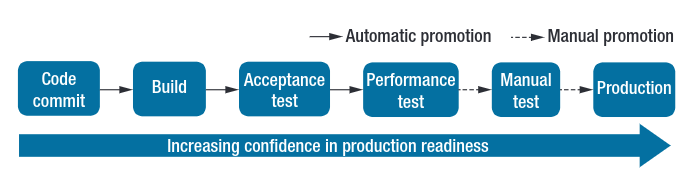
\includegraphics[width=1\textwidth]{figures/continouse-delivery-pipeline.png}
    \caption{Contoh pipeline dalam Continous Delivery}
\end{figure}

\subsection{Metode Continuous Deployment}
Perbedaan mendasar dari Continuous Delivery (CDE) dan Continuous Deployment (CD) adalah dimana implementasi semua fase
dilakukan secara automatis tanpa memerlukan intervensi manusia, deployment
ke tahap environment produksi juga bisa dilakukan secara automatis, tetapi biasanya memerlukan intervensi pada satu tahap \cite{Ramadoni2021}.
\vspace{0.5cm}
\section{Deployment Pada Kubernetes}
Pada padasarnya terdapat 2 metode yang digunakan untuk melakukan
deployment pada sebuah aplikasi pada kubernetes yaitu pull method dan push method \cite{Ramadoni2021}.
Perbedaan  mendasar dari pull method dan push method terdapat pada agent yang melakukan
deployment \cite{GitOps}. Pada push method sebuah agent melakukan deployment sebuah  service terhadap suatu platform (eg, kubernetes).
\vspace{0.5cm}
\subsection{Push-based Deployment}
Push-based deployment \cite{GitOps} merupakan strategy yang popular yang diimplementasikan oleh
tools seperti Jenkins, CircleCI, atau TravisCI.
Sourcecode dari sebuah aplikasi terdapat pada repository yang sama dengan konfigurasi YAML Kubernetes yang diperlukan untuk melakukan deployment aplikasi tersebut.
Kapan pun code dari aplikasi tersebut diupdat, pipeline akan berjalan, dimana akan membuat container image yang diperlukan.
Perlu diperhatikan juga bahwa biasanya credential environment untuk melakukan deployment pada metode Push-based. Jadi pada pipeline tersebut kita dapat melihat
configurasi rahasia yang mungkin saja terlihat oleh orang lain.
\begin{figure}[ht]
    \centering
    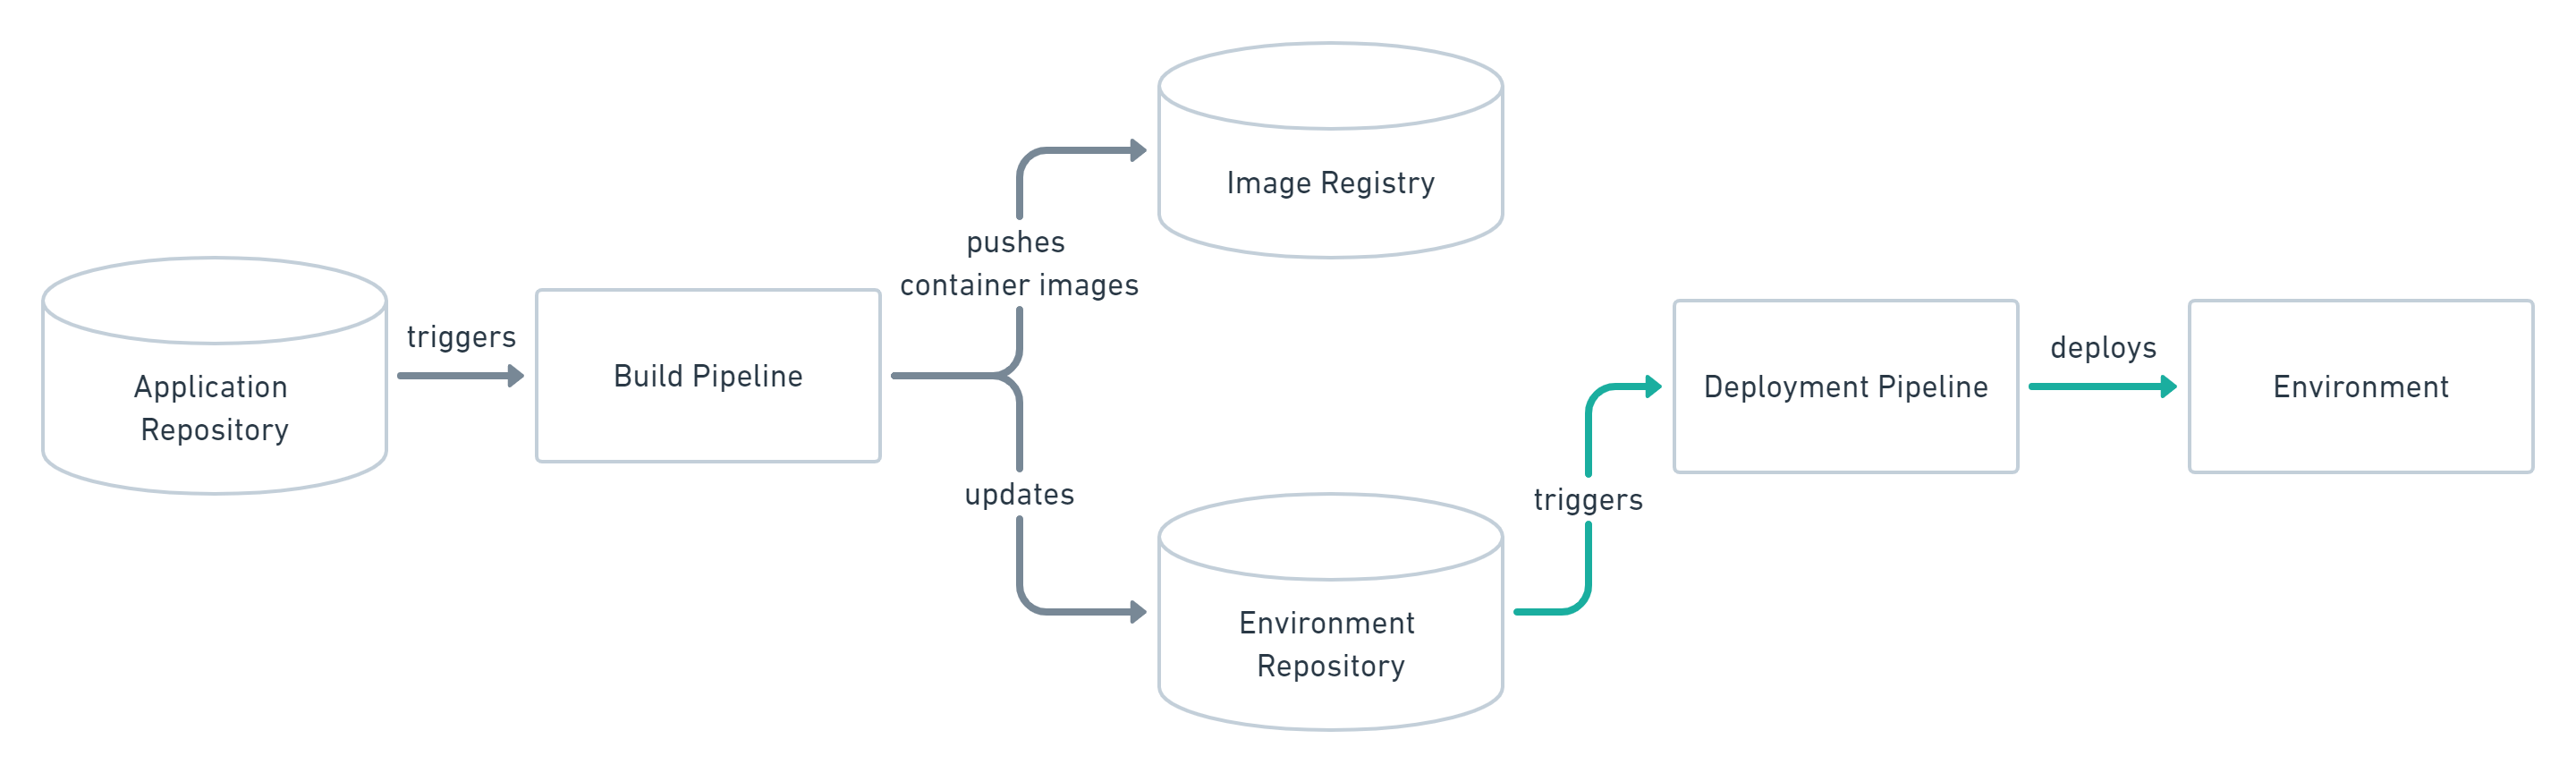
\includegraphics[width=1\textwidth]{figures/push-based.png}
    \caption{Contoh pipeline dalam push-based deployment}
\end{figure}
\newpage
\vspace{0.5cm}
\subsection{Pull-based Deployment}
Pada website insert gitops Strategi Pull-based deployment menggunakan konsep
yang sama dengan push-based tetapi berbeda pada bagaimana cara kerja pada pipeline deployment.
Secara traditional pipeline CI/CD akan di-trigger oleh event eksternal, contohnya ketika ada update kode
baru yang pada repository. Dengan metode pull-based deployment, dikenalkan sebuah operator.
Operator tersebut secara kontinu dengan interval yang dapat diatur sendiri melakukan komparasi
terhadap state yang ada di repository dengan state yang ter-deploy pada infrastructure.
Ketika terdapat perbedaan, operator melakukan update pada infrastructure untuk mencocokan state dengan apa yang ada di repository.
Operator harus berada pada environment atau kluster yang sama dengan applikasi yang akan dideploy. Dengan ini pull-based method
tidak perlu mengetahui environment eksternal karena semua sudah ada pada kluster yang sama.
\begin{figure}[h]
    \centering
    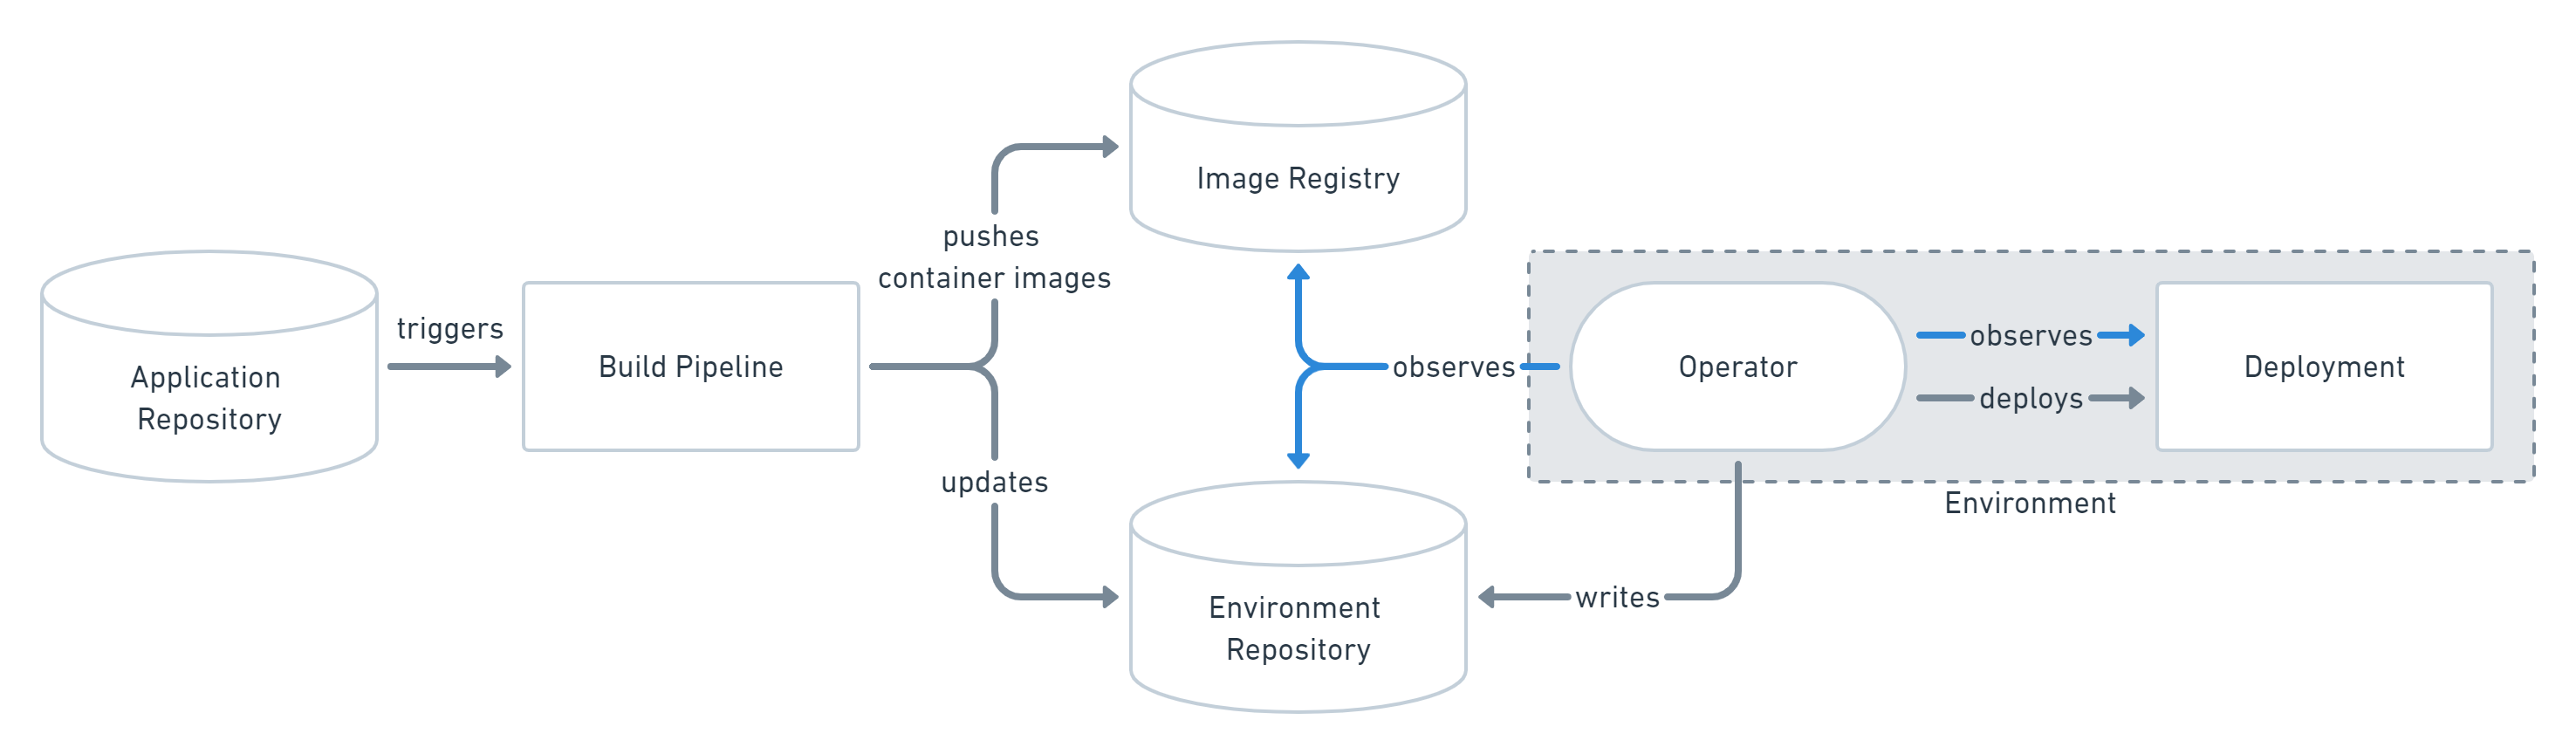
\includegraphics[width=1\textwidth]{figures/pull-based.png}
    \caption{Contoh pipeline dalam pull-based deployment}
\end{figure}
\vspace{0.5cm}

\newpage
\section{Arsitektur Cluster Kubernetes yang akan digunakan}
Dibawah ini merupakan rancangan arsitektur high-level pada implementasi Kubernetes
nantinya. Disini menggunakan Metal-LB sebagai provider load  balancer dan Traefik sebagai ingress controller.
\begin{figure}[h]
    \centering
    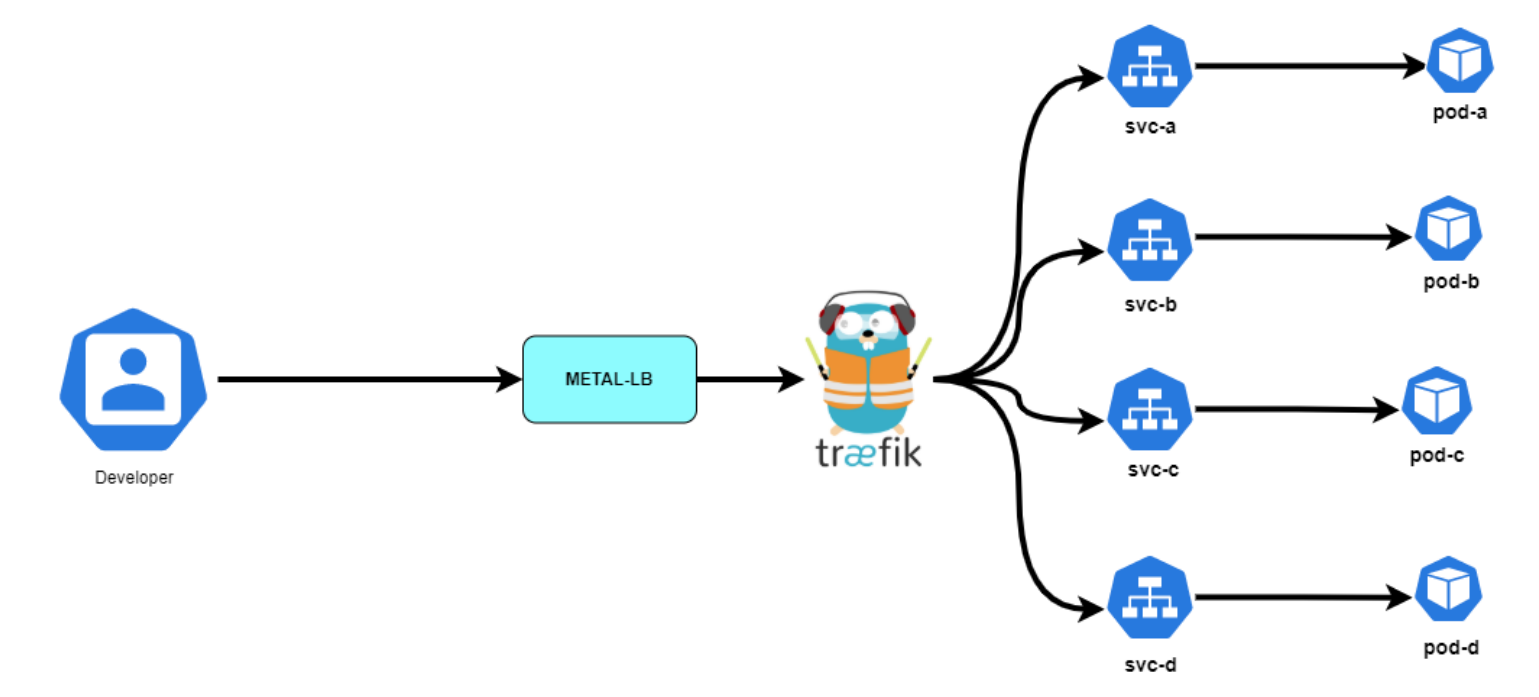
\includegraphics[width=1\textwidth]{figures/kubernetes-arch.png}
    \caption{Arsitektur Kubernetes yang akan digunakan}
\end{figure}
\newpage